%%%%%%%%%%%%%%%%%%%%%%%%%%%%%%%%%%%%%%%%%%%%%%%%%%%%%%
% A Beamer template for HKUST (GZ)                   %
% Based on THU beamer theme                          %
% Author: Yuxuan HU                                  %
% Date: Aug 2024                                    %
% LPPL Licensed.                                     %
%%%%%%%%%%%%%%%%%%%%%%%%%%%%%%%%%%%%%%%%%%%%%%%%%%%%%%

\documentclass[aspectratio=169]{beamer}
\usefonttheme{serif}

%\documentclass[serif]{beamer}  % for 4:3 ratio
\usepackage[T1]{fontenc} 
\usepackage{fourier} % see "http://faq.ktug.org/wiki/uploads/MathFonts.pdf" for other options
\usepackage{hyperref}
\usepackage{latexsym,amsmath,xcolor,multicol,booktabs,calligra}
\usepackage{graphicx,pstricks,listings,stackengine}
\usepackage{lipsum}
\usepackage{comment}


\author{Jordan Dutel}
\title{M2 Bio-Informatic Internship}
\subtitle{10/06/2025 Presentation}
\institute{
    Université Claude Bernard Lyon 1 \\
    Centre de Recherche en Cancérologie de Lyon (CRCL) \\
    Team : Dr Pierre Saintigny \\
    Tutor : Dr Pierre Martinez \\
}
\date{\small \today}
\usepackage{HKUSTstyle}

% defs
\def\cmd#1{\texttt{\color{red}\footnotesize $\backslash$#1}}
\def\env#1{\texttt{\color{blue}\footnotesize #1}}
\newcommand{\figpath}{/mnt/datadisk/Jordan/Delivrables/Rapports/Rapport_stage/Figures/Sans_légendes}
\newcommand{\imagesource}[1]{%
    \vspace{0.1cm}
    \begin{flushright}
    \tiny\color{gray}#1
    \end{flushright}
}




% set colors
\definecolor{hkustyellow}{RGB}{167, 131, 55}
\definecolor{hkustblue}{RGB}{0, 56, 116}
\definecolor{hkustred}{RGB}{209, 51, 59}


\lstset{
    basicstyle=\ttfamily\small,
    keywordstyle=\bfseries\color{deepblue},
    emphstyle=\ttfamily\color{deepred},    % Custom highlighting style
    stringstyle=\color{deepgreen},
    numbers=left,
    numberstyle=\small\color{halfgray},
    rulesepcolor=\color{red!20!green!20!blue!20},
    frame=shadowbox,
}

\setbeamertemplate{navigation symbols}{} % Permet d'enlever la barre d'outils en bas à droite de chaque diapos

%- --- --- --- --- --- --- --- --- --- --- --- --- --- --- --- 
\begin{document}





\begin{frame}
    \titlepage
    \vspace*{-0.6cm}
    \begin{center}
        \begin{minipage}{0.3\textwidth}
            \centering
            
\includegraphics[scale=0.125]{Logos/bioinfo_lyon1.png}
        \end{minipage}
        \begin{minipage}{0.3\textwidth}
            \centering
            
\includegraphics[scale=0.01]{Logos/ucbl-logo-ucbl.png}
        \end{minipage}
        \begin{minipage}{0.3\textwidth}
            \centering
            
\includegraphics[scale=0.10]{Logos/Logo_CRCL.png}
        \end{minipage}
    \end{center}
\end{frame}


\begin{comment}

\begin{frame}    
    \tableofcontents[sectionstyle=show,
    subsectionstyle=show/shaded/hide,
    subsubsectionstyle=show/shaded/hide]
\end{frame}

\end{comment}


% Introduction --- --- --- --- --- --- --- --- --- --- --- --- 
\section{Introduction}

\begin{frame}{Context}
    \frametitle<presentation>{Context}
    
    \begin{figure}[h]
        \centering
        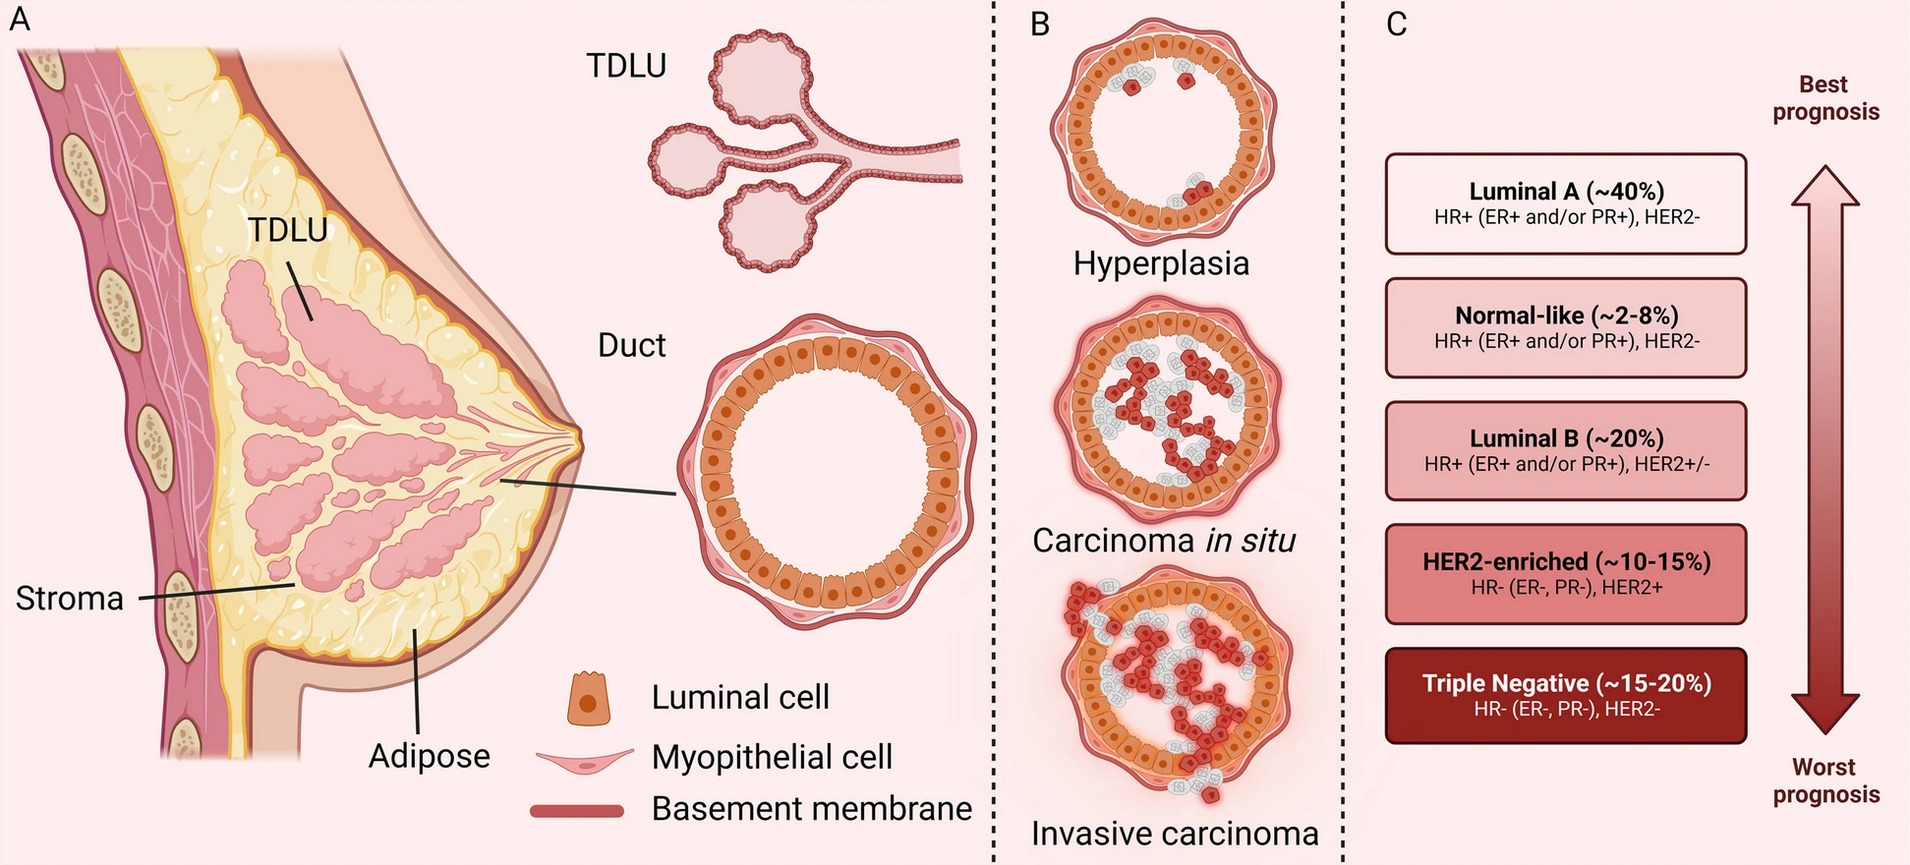
\includegraphics[width=\textwidth, height=5.5cm]{Images/Fig_expli.png}
        % Ligne en bas : à gauche les abréviations, à droite la source
        \begin{minipage}{0.48\textwidth}
            \raggedright
            \tiny \color{gray}
            TNBC: Triple-Negative Breast Cancer\\
            TDLU: Terminal Duct Lobular Units
        \end{minipage}%
        \hfill
        \begin{minipage}{0.48\textwidth}
            \raggedleft
            \tiny \color{gray} Source: Chang-Yun Li \\ \href{https://molecular-cancer.biomedcentral.com/articles/10.1186/s12943-024-02011-0}{biomedcentral.com} (CC BY 4.0)
        \end{minipage}

        \centering
        \textbf{MpBC (Metaplastic Breast Carcinomas) are rare forms of TNBC, \\lacking molecular diagnostic markers and specific therapies}
    \end{figure}
\end{frame}

\begin{frame}{Trans-differenciation}
    \frametitle<presentation>{Trans-differenciation}
    
    \begin{figure}[h]
        \centering
        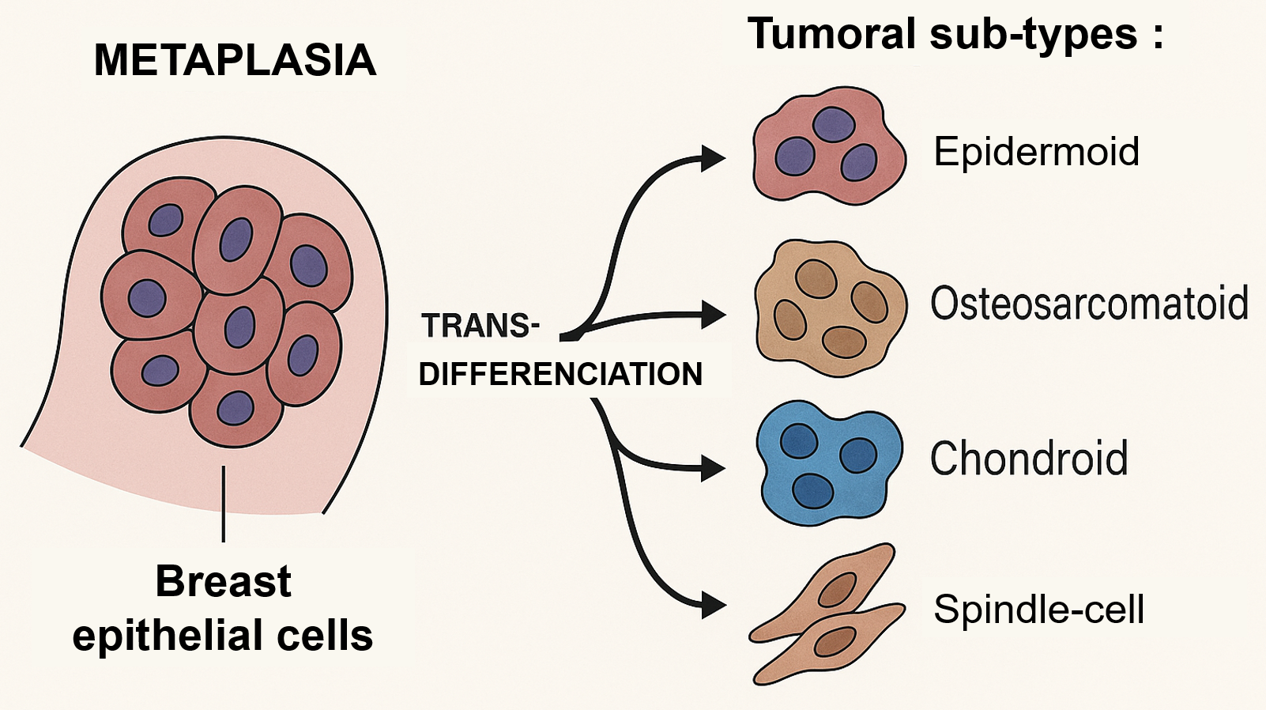
\includegraphics[width=0.80\textwidth, height=5.5cm]{\figpath/Transdiff.png}\\
        \centering
        \textbf{MpBC can transdifferentiate into various aggressive tumor subtypes}
    \end{figure}
\end{frame}

\begin{frame}{Trans-differentiation}
    \frametitle{Trans-differentiation}

    \begin{figure}
        \centering
        \begin{minipage}{0.48\textwidth}
            \small
            \begin{itemize}
                \item \textbf{MpBC} exhibits a remarkable \textbf{plasticity} \\
                \item \textbf{Transdifferenciation} into multiple aggressive \textbf{tumor subtypes}\\
                \item \textbf{Mixed MpBC}
                    \begin{itemize}
                        \item Each sample contains \textbf{at least 2 tumoral compartments}
                    \end{itemize}
            \end{itemize}
        \end{minipage}
        \hfill
        \begin{minipage}{0.48\textwidth}
            \centering
            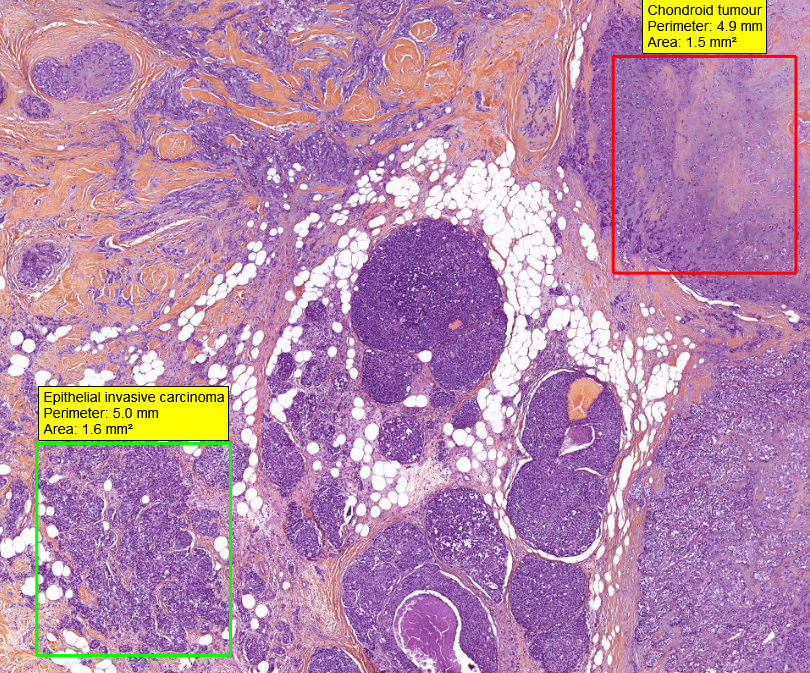
\includegraphics[width=\textwidth, height=5.5cm]{Images/TransDiff_sample.png}
        \end{minipage}
        
    \end{figure}
\end{frame}








\begin{frame}{Research questions}

    \begin{block}{Unresolved questions}
        \begin{enumerate}
            \item Understanding the \textbf{evolutionary trajectories} in MpBC.
            \begin{itemize}
                \item Internal determinants (genetic and epigenetic)
                \item External determinants (tumor microenvironment)
            \end{itemize} 
            \item Identify molecular biomarkers to \textbf{improve diagnostic} precision.
            \item Discover genetic and epigenetic features that may serve as potential \textbf{therapeutic targets}.
        \end{enumerate}
    \end{block}

    \vspace{0.5cm}

    \begin{block}{Internship Aims}
        \begin{itemize}
            \item Determine \textbf{expression markers} specific to different tumor sub-types.
            \item Analyze \textbf{genomic divergence} between tumoral compartments.
        \end{itemize}
    \end{block}
    
\end{frame}



\begin{frame}{Data available}
    \frametitle{Data}

    \begin{minipage}{0.58\textwidth}
        \begin{itemize}
            \item \textbf{Spatial transcriptomic counts} (\emph{Visium}, 10X Genomics)
            \item \textbf{16 mixed MpBC} samples
            \item Different tumor \textbf{transdifferentiation} states captured
        \end{itemize}
    \end{minipage}
    \hfill
    \begin{minipage}{0.4\textwidth}
        \centering
        \includegraphics[width=\textwidth, height=4.5cm]{\figpath/sample_no_annot.png}
        \vspace{0.3em}
    \end{minipage}
\end{frame}





\begin{frame}{MpBC sample}
    \centering
    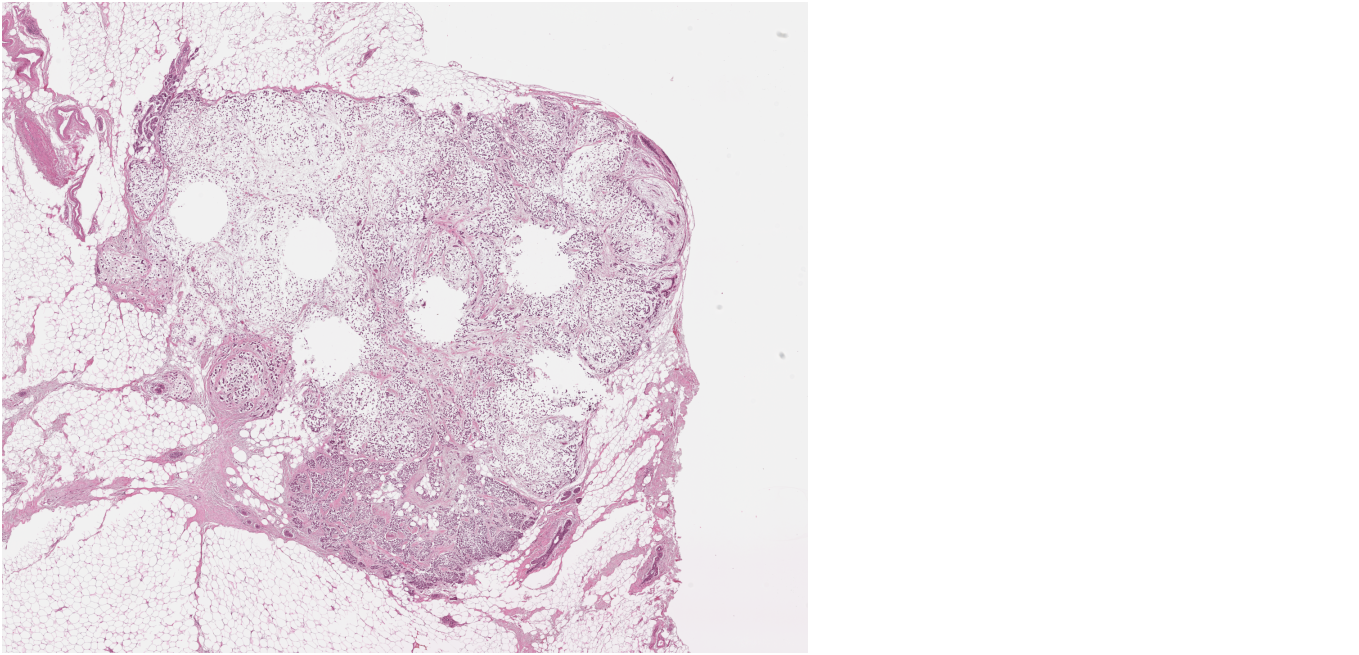
\includegraphics[width=\textwidth, height=5.5cm]{\figpath/MpBC9_tissue.png}
    \vspace{0.82cm}
\end{frame}

\begin{frame}{Expert annotations}
    \centering
    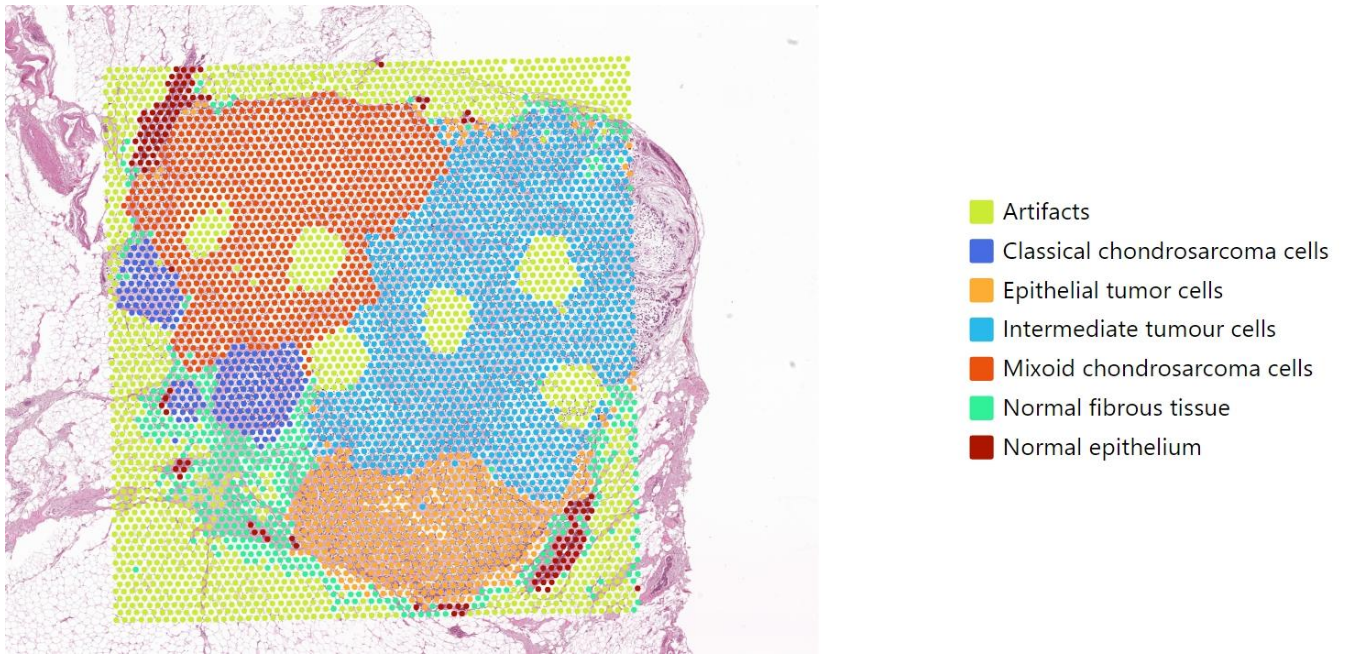
\includegraphics[width=\textwidth, height=5.5cm]{\figpath/MpBC9_tissue_annot.png}

    \vspace{0.3cm} % petit espace pour séparer image et texte sans décaler l'image
    \textbf{Mixed MpBC} with several tumor cell types covered by \textbf{Visium spots},\\
    \textbf{grouped by k-means clustering} and \textbf{annotated by a pathologist}.
\end{frame}




% Pipeline --- --- --- --- --- --- --- --- --- --- --- 
\begin{comment}


\section{Workflow}

\begin{frame}{Pipeline}
    \begin{block}{Steps}
        \begin{multicols}{2}
            \begin{enumerate}
                \item Load data
                \item Merging objects
                \item Normalisation
                \item PCA
                \item Harmony (Batch effect correction)
                \item UMAP
                \item Find cell-clusters
                \item Find cluster-specific markers
            \end{enumerate}
        \end{multicols}
    \end{block}

    \begin{block}{Tools}
        \begin{table}[h]
            \centering
            \begin{tabular}{|c|c|c|}
                \hline
                \textbf{Step} & \textbf{R Packages/Functions} \\
                \hline
                Read Data & Seurat \\ 
                Normalization & NormalizeData() + ScaleData() (No SCTransform !!!)\\
                Batch effect correction & RunHarmony() \\
                \hline
            \end{tabular}
        \end{table}
    \end{block}
\end{frame}


\end{comment}








% Results --- --- --- --- --- --- --- --- --- --- --- 
\section{Results}
\subsection{Phenotypic markers analysis}


\begin{comment} 
\begin{frame} % [plain] enlève l'en-tête et le pied de page
    \centering
    \vspace{2cm}
    {\LARGE \textbf{Results}}\\[1.5em]
    
    {\Large Part I: Phenotypic Marker Analysis}\\[0.8em]
    {\Large Part II: CNA Analysis}
\end{frame}
\end{comment}

\begin{frame}
	\frametitle<presentation>{Batch effect correction : Harmony}
	\begin{figure}
		\centering
			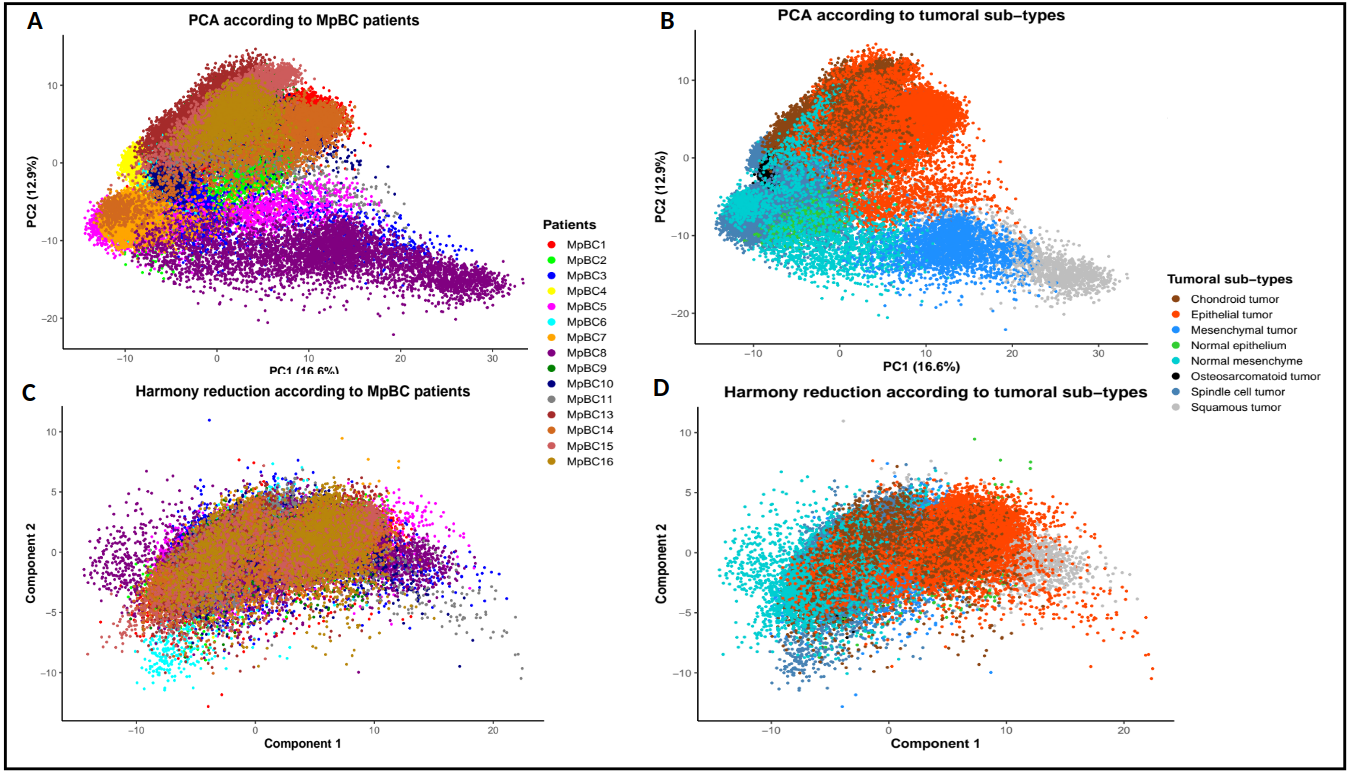
\includegraphics[width=\textwidth, height=6.5cm]{\figpath/Fig2_remix.png}\\
            \centering
            \textbf{Improve integration with fewer isolated patients}
        % Bonne separation épi-mes (moins bien intra mes)
		\label{fig:harmony_tumor_cell_types}
	\end{figure}
\end{frame}

\begin{frame}
	\frametitle<presentation>{UMAP Projection}
	\begin{figure}
		    \centering
			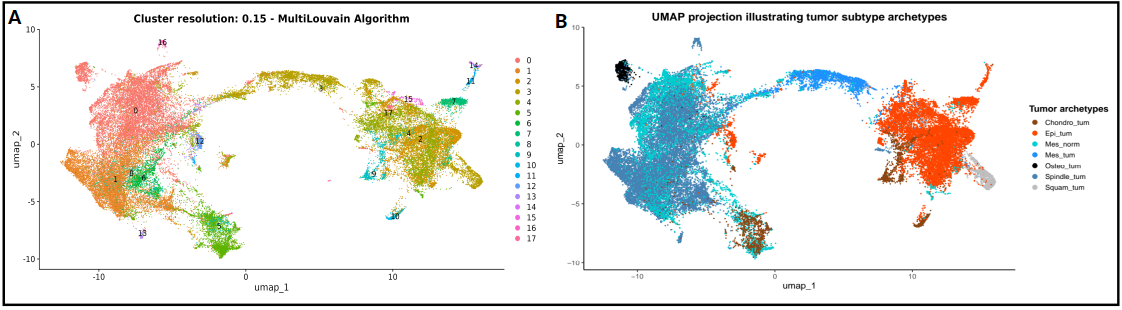
\includegraphics[width=14cm, height=5cm]{\figpath/cluster_umap.png}\\
            \centering
            \textbf{Clear epithelial-mesenchymal axis (umap1), with few ambiguous spots}
            \label{fig:umap}
	\end{figure}
\end{frame}


\begin{comment}
\begin{frame}
	\frametitle<presentation>{UMAP Projection}
	\begin{block}{Points to discuss}
        \begin{itemize}
    	    \item Some points/cells are still patient-specific (Chondroid and Epithelial cells).
                \begin{itemize}
                    \item Enhance Harmony correction (but jeopardize biological signal) ?
                \end{itemize}
            \item Chondroid cells difficult to regroup and Spindle cells really heterogenous...
        \end{itemize}
    \end{block}
    \begin{block}{Solutions}
        \begin{itemize}
            \item Single nuclei and spot deconvolution to improve cell groups according to cell types/annotations
        \end{itemize}
    \end{block}
\end{frame}

\begin{frame}
	\frametitle<presentation>{Clustering}
	\begin{block}{Points to discuss}
        \begin{itemize}
    	    \item Mesenchymal tumor cluster close to Squamous tumor... 
                \begin{itemize}
                    \item Strange, because phenotypically very different
                    \item Come from the same patient (MpBC8)
                    \item Harmony correction not enough ?
                \end{itemize} 
            \item Some clusters are still patient-specific more than cell-types-specific (e.g. Epi-tum)
        \end{itemize}
    \end{block}
\end{frame}
\end{comment}


\begin{frame}
	\frametitle<presentation>{Expression markers}
	\begin{figure}
		\centering
			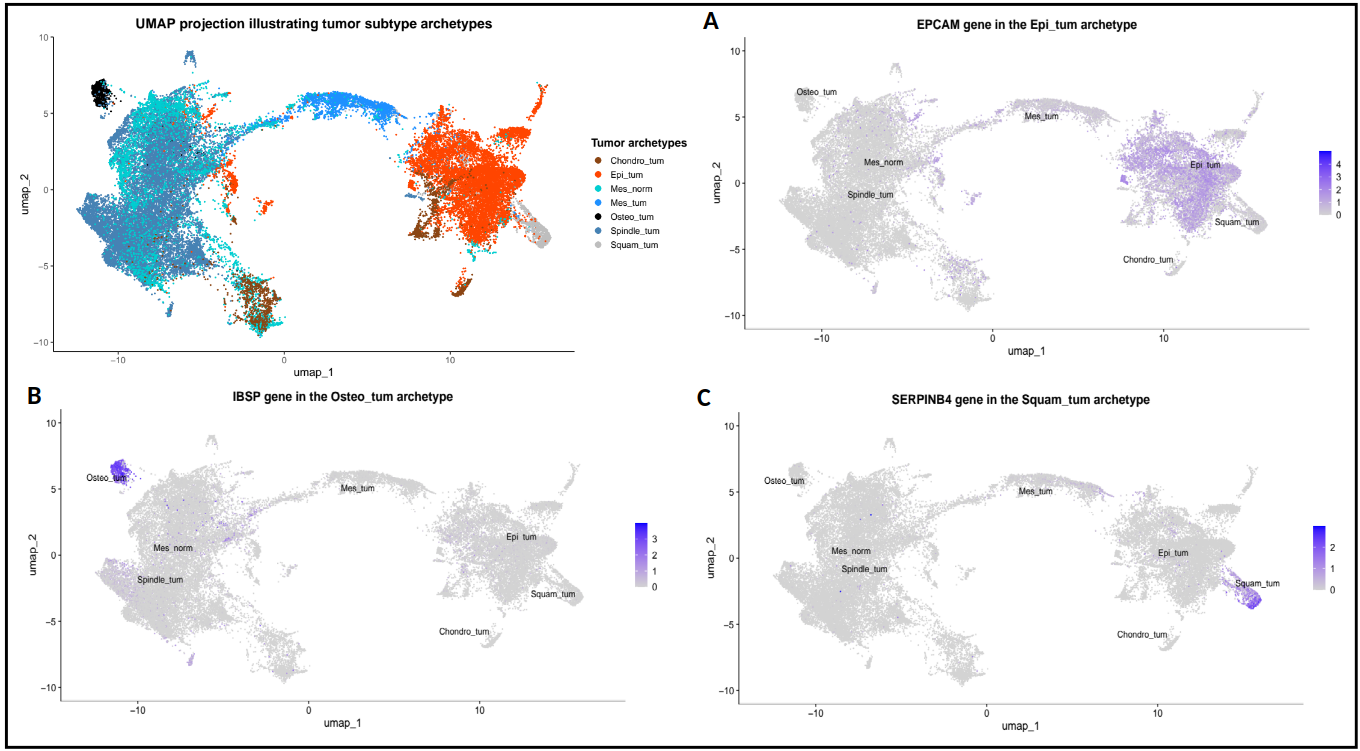
\includegraphics[width=\textwidth, height=6cm]{\figpath/Fig4_remix_abc.png}\\
            \centering
            Analysis with \textbf{MAST} (Model-based Analysis of Single-cell Transcriptomics)\\
            \textbf{Some phenotypic markers identified are specific to clusters...}
		\label{fig:4bis1}
	\end{figure}
\end{frame}

\begin{frame}
	\frametitle<presentation>{Expression markers}
	\begin{figure}
		\centering
			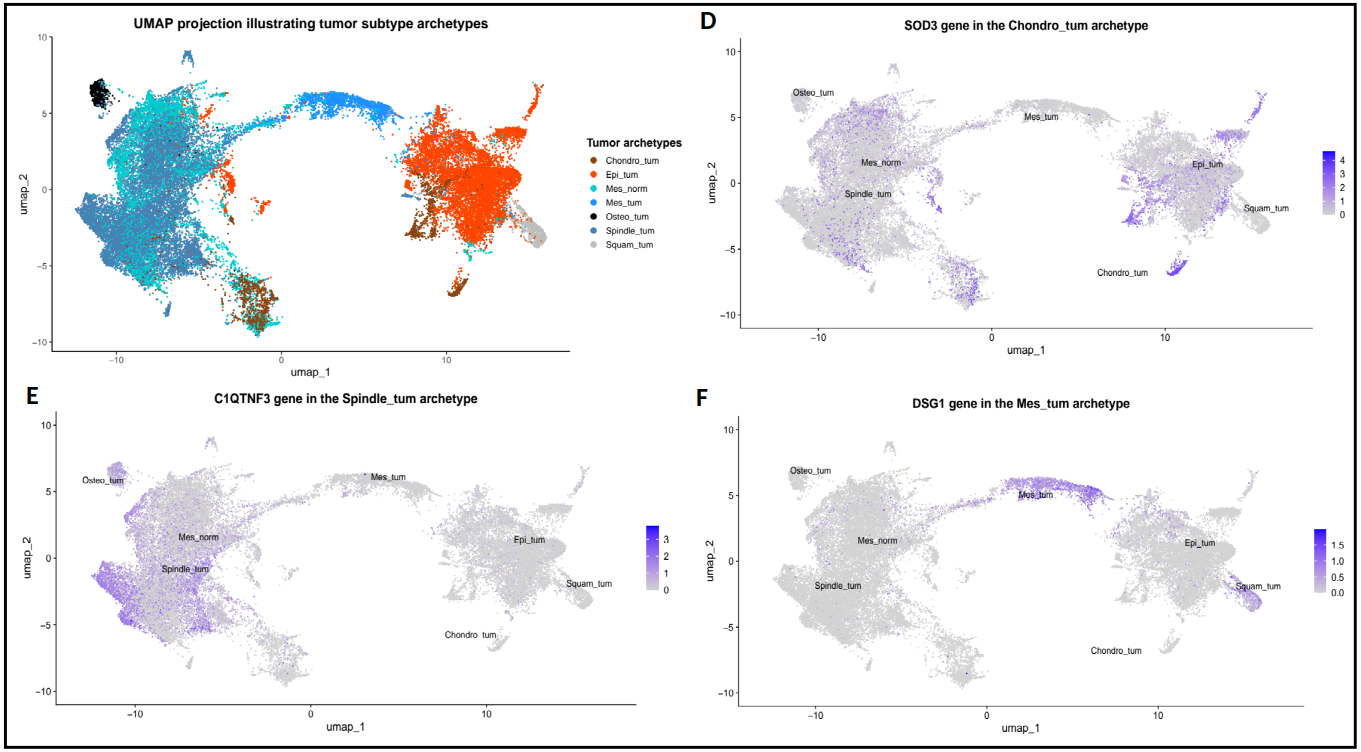
\includegraphics[width=\textwidth, height=6cm]{\figpath/Fig4_remix_def.png}\\
            \centering
            \textbf{Few phenotypic markers aren't specific  enough (Visium limitations)}\\
            Different \textbf{spot purity} depending on the \textbf{subtypes}
		\label{fig:4bis2}
	\end{figure}
\end{frame}

\begin{comment}
\begin{frame}
	\frametitle<presentation>{Markers specificities}
	\begin{figure}
		\centering
			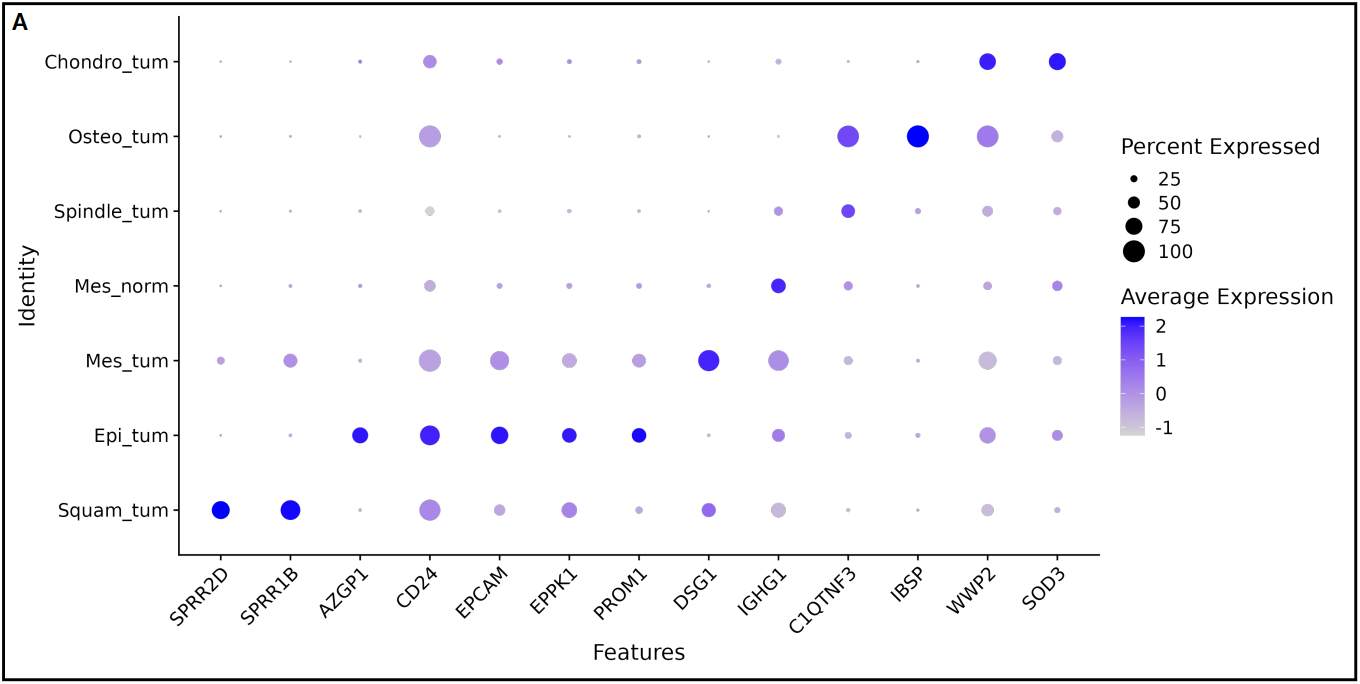
\includegraphics[width=\textwidth, height=6cm]{\figpath/Fig5_a.png}
            \centering
            \textbf{Some markers seems to be overexpressed only in specific clusters...}\\
		\label{fig:dotplot_clusters}
	\end{figure}
\end{frame}
\end{comment}

\begin{frame}
	\frametitle<presentation>{Markers specificities}
	\begin{figure}
		\centering
			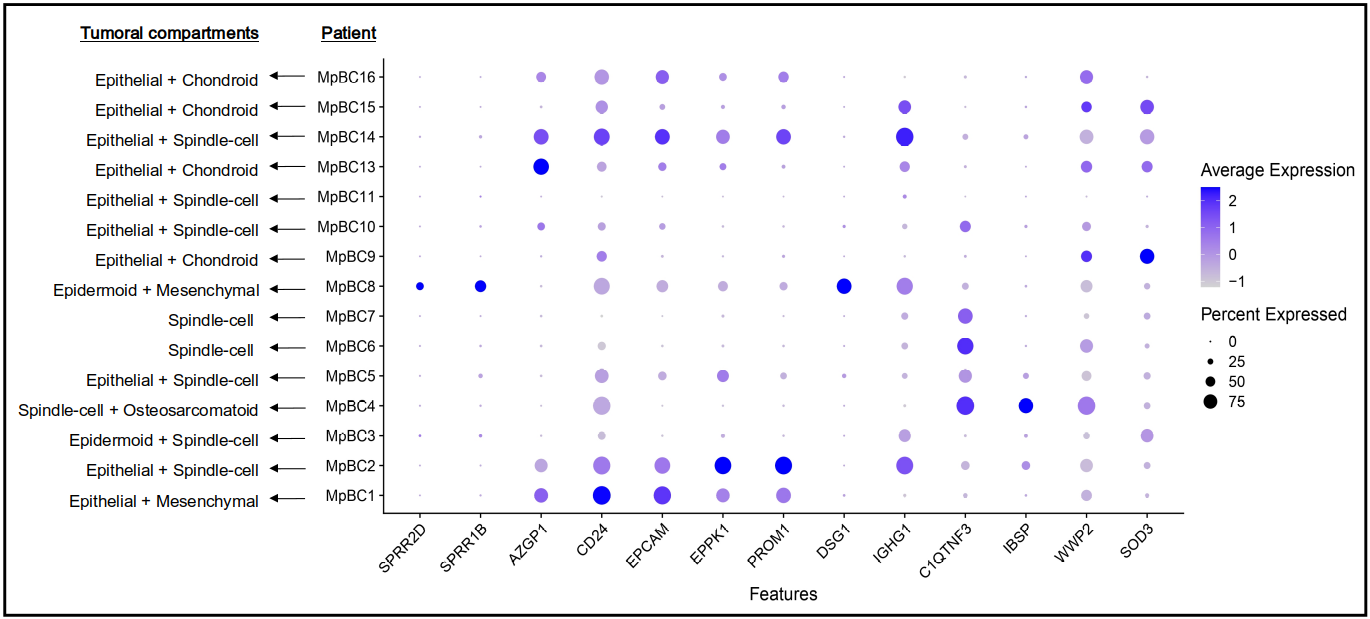
\includegraphics[width=\textwidth, height=6cm]{\figpath/Fig5_b_remix.png}
            \centering
            \textbf{Some cluster-specific markers are also patient-specific markers}
		\label{fig:dotplot_clusters2}
	\end{figure}
\end{frame}

\begin{frame}{Analysis conclusions}

    \begin{itemize}
        \item Analysis reveals \textbf{archetype-specific markers}
            \begin{itemize} 
                \item \textbf{Epidermoid}
                \item \textbf{Epithelial}
                \item \textbf{Osteosarcomatoid}
            \end{itemize}
        \item Some markers remain \textbf{non-specific or not representative of the archetypes}
            \begin{itemize} 
                \item \textbf{Spindle-cell}
                \item \textbf{Chondroid}
                \item \textbf{Mesenchymal}
            \end{itemize}
        \item \textbf{Spatial transcriptomics} combined with \textbf{pathologist annotations} is \textbf{promising}, but \textbf{still limited} by the \textbf{cellular purity of Visium spots}.
    \end{itemize}
    
\end{frame}






\subsection{Copy Number Alterations (CNA) analysis}



  

\begin{comment}
\begin{frame}
	\frametitle<presentation>{Chromosomic arms and cytobands}
	\begin{figure}
        \begin{minipage}{0.48\textwidth}
            \raggedleft

            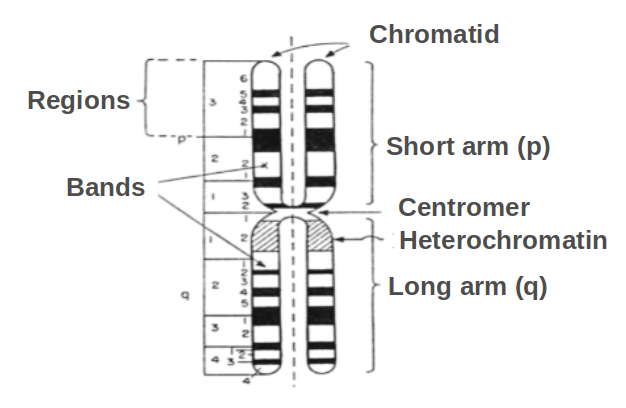
\includegraphics[width=1.2\textwidth, height=6cm]{\figpath/cytobands_chrom.png}\\
        \end{minipage}


        \begin{minipage}{0.48\textwidth}            
            \raggedleft
            \tiny \color{gray} Source: Axel Feraut \href{https://cdn.unilim.fr/files/theses-exercice/P20113359.pdf}{cdn.unilim.fr}
		\end{minipage}

        \centering
        \textbf{Each chromosome arm (p and q) consists of a series of cytoband}
        \label{fig:chrom_cyto}
	\end{figure}
\end{frame}
\end{comment}

\begin{frame}{CNA in cancer}
    \begin{itemize}
        \item \textbf{Frequent in cancer:} CNA are a hallmark of cancer cells.
        \vspace{0.5em}
        
        \item \textbf{Types of alterations:}
        \begin{itemize}
            \item Can be \textbf{focal} (targeting specific genes or regions)
            \item Or \textbf{broad}, affecting entire cytobands or chromosome arms
        \end{itemize}
        \vspace{0.5em}
        
        \item \textbf{Functional impact:} 
        \begin{itemize}
            \item CNA can lead to oncogene amplification or tumor suppressor loss
        \end{itemize}
        \vspace{0.5em}

        \item \textbf{Clonal evolution insight:}
        \begin{itemize}
            \item CNA profiles help reconstruct \textbf{evolutionary trajectories}
            \item Reveal selection of clones and subclones in tumor
        \end{itemize}
    \end{itemize}
\end{frame}

\begin{frame}
	\frametitle<presentation>{Raw InferCNVPlus results}
	\begin{figure}
		\centering
			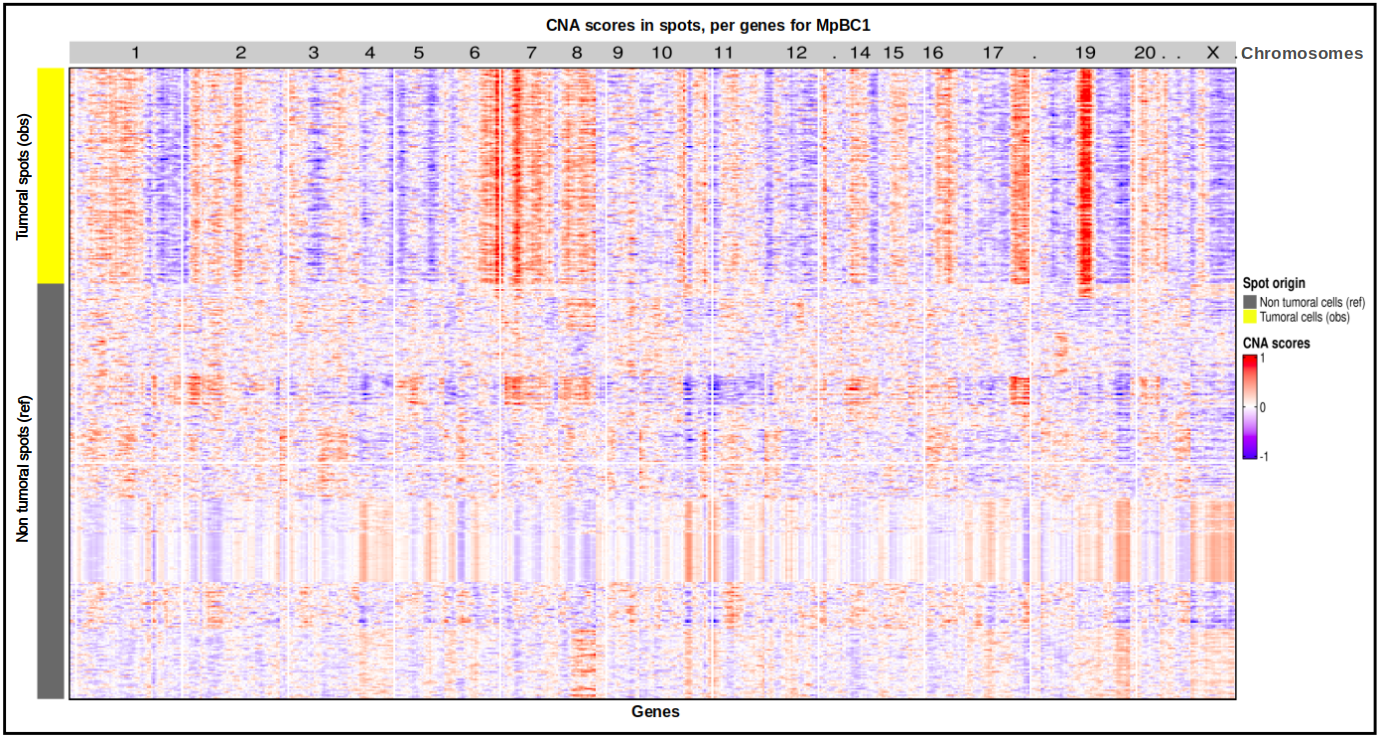
\includegraphics[width=\textwidth, height=6cm]{\figpath/Raw_Infer.png}\\
            \centering
            \textbf{Raw CNA scores in tumoral (obs) or non tumoral (ref) spots for each gene expressed}
		\label{fig:heatmap1}
	\end{figure}
\end{frame}

\begin{frame}
	\frametitle<presentation>{Heatmap}
	\begin{figure}
		\centering
			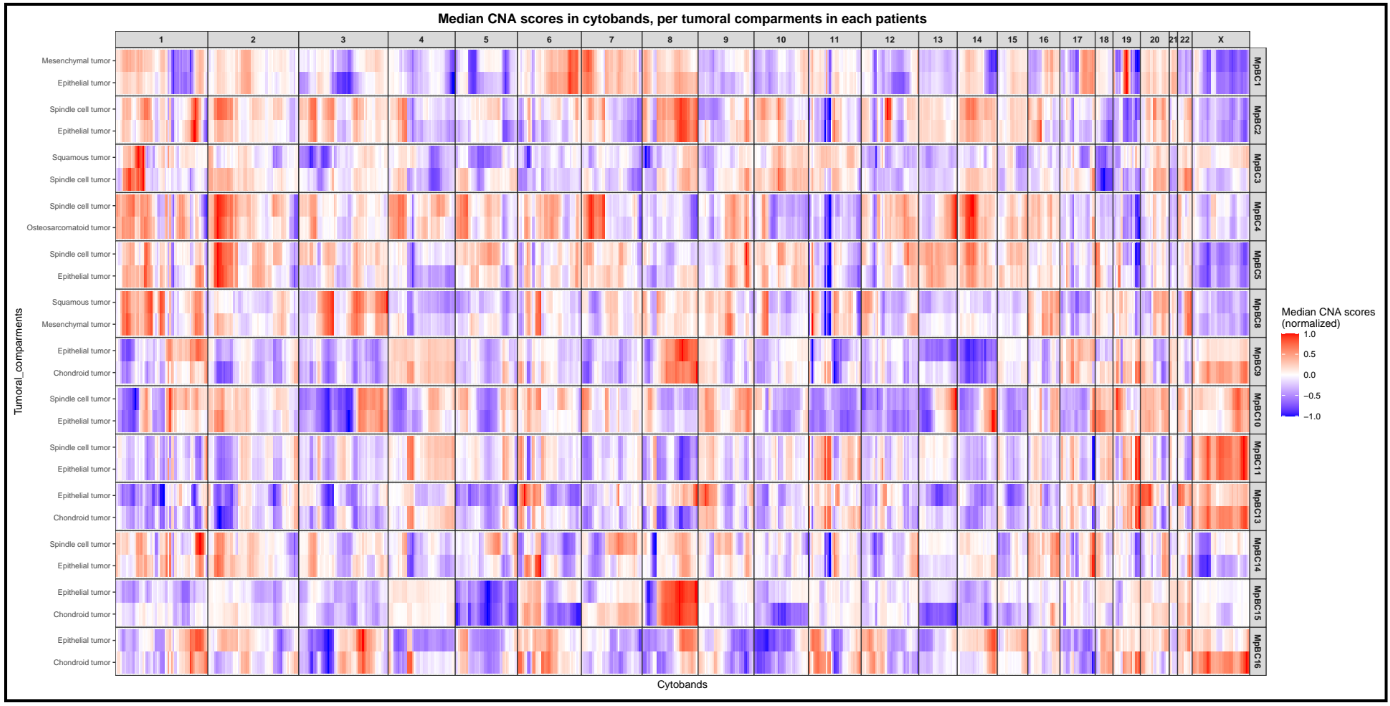
\includegraphics[width=\textwidth, height=6cm]{\figpath/Heatmap_all.png}\\
            \centering
            \textbf{CNA scores in each tumoral compartments for each cytoband}
		\label{fig:heatmap2}
	\end{figure}
\end{frame}

\begin{frame}
	\frametitle<presentation>{RNA sequencing depth per spot}
	\begin{figure}
		\centering
            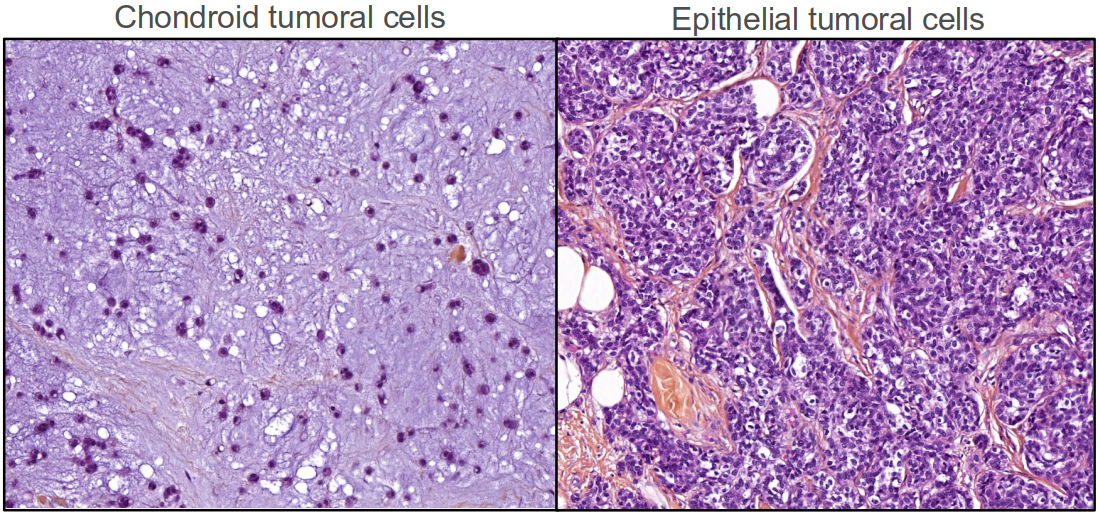
\includegraphics[width=\textwidth, height=5.5cm]{\figpath/Spot_depth.png}\\
            \centering
            \textbf{Normalization to correct for differences in RNA sequencing depth across spots}
		\label{fig:depth}
	\end{figure}
\end{frame}

\begin{frame}
	\frametitle<presentation>{Genomic CNA profil}
	\begin{figure}
		\centering
			\includegraphics[width=0.85\textwidth, height=6.5cm]{\figpath/Fig6_remix.png}\\
            \centering
            \textbf{Some genomic regions are higly altered even after the normalisation}
		\label{fig:shiftplot}
	\end{figure}
\end{frame}

\begin{comment}
\begin{frame}
	\frametitle<presentation>{Statistical tests}
	\begin{figure}
		\centering
			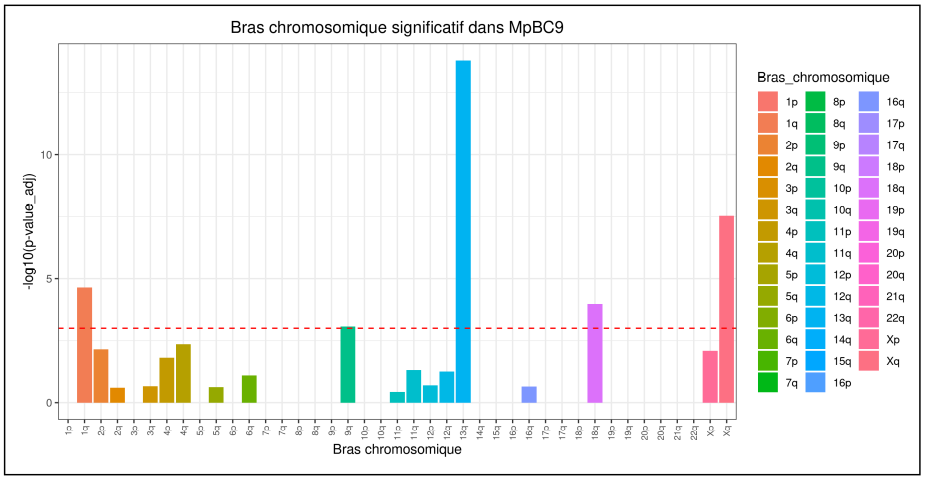
\includegraphics[width=\textwidth, height=5.5cm]{\figpath/Fig7.png}\\
            \centering
            \textbf{Statistical testing by chromosomic arms reveal several regions significatively altered}
		\label{fig:barplot}
	\end{figure}
\end{frame}
\end{comment}





\begin{frame}
	\frametitle<presentation>{VolcanoPlot}
	\begin{figure}
		\centering
			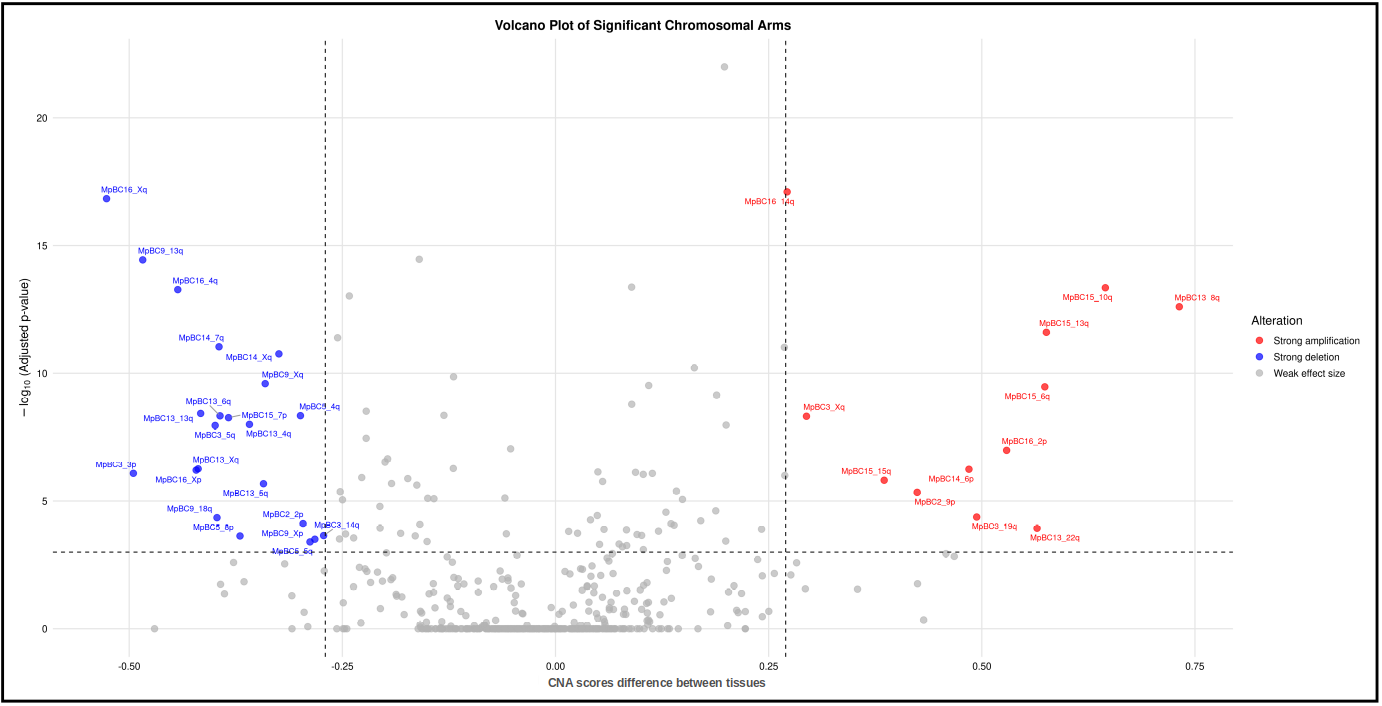
\includegraphics[width=\textwidth, height=6.5cm]{\figpath/Volcano.png}\\
            \centering
            \textbf{Some chromosomic arms significatively altered for few patients}
		\label{fig:all-arms}
	\end{figure}
\end{frame}

\begin{frame}
	\frametitle<presentation>{Correlation Plot}
	\begin{figure}
		\centering
			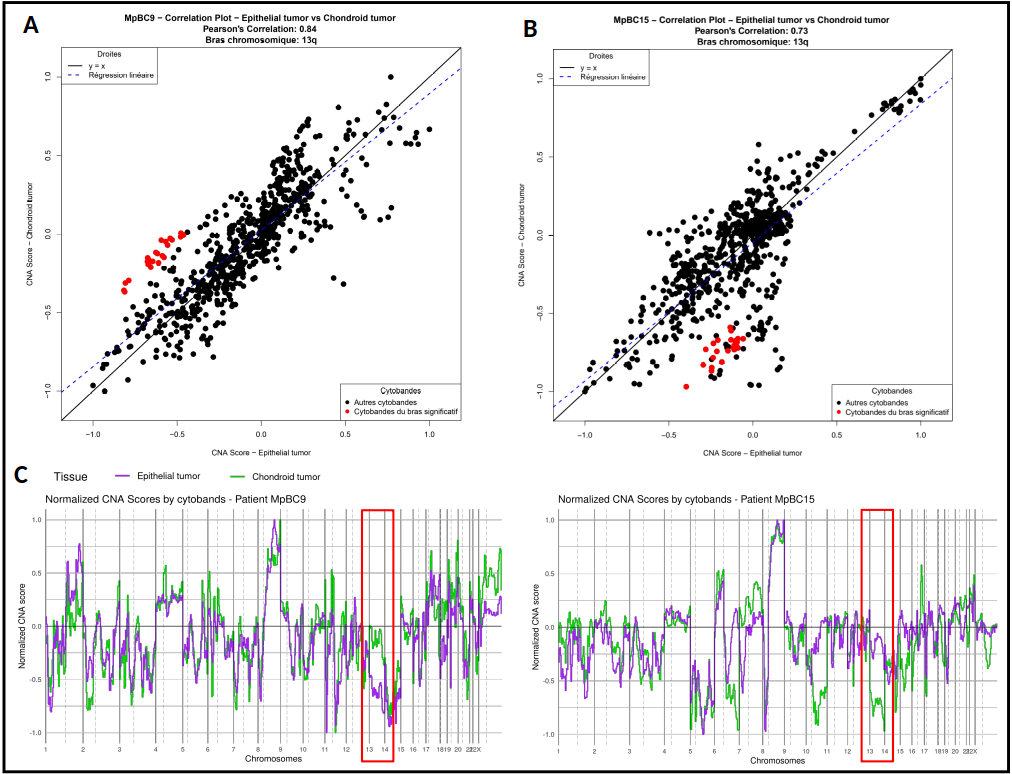
\includegraphics[width=0.8\textwidth, height=6.5cm]{\figpath/Corrplot_remix.png}\\
            \centering
            \textbf{Significant cytobands deviate from other cytoband distributions}
		\label{fig:corrplot}
	\end{figure}
\end{frame}

\begin{frame}{Analysis Conclusions}
    \begin{itemize}
        \item \textbf{Limited divergence} in CNA profiles between paired tumor compartments  
        \begin{itemize} 
            \item Suggests a \textbf{shared clonal origin} for tumor subtypes
        \end{itemize}
        \vspace{0.5cm}
        \item \textbf{Rare cases} of chromosomal arm-level divergence between compartments  
        \begin{itemize} 
            \item May reflect \textbf{subclonal evolution}, where one compartment originates from the other
        \end{itemize}
    \end{itemize}
\end{frame}


% Conclusions --- --- --- --- --- --- --- --- --- --- --- 
\section{Conclusions}

\begin{comment} 
\begin{frame}{Conclusion}
    \begin{block}{Main goal}
        \begin{itemize}
            \item Identify \textbf{genes involved} in transdifferentiation and specific to each tumor subtype.
            \item Identify \textbf{genomic alterations (e.g., CNAs)} potentially driving transdifferentiation and specific to each tumor subtype.
        \end{itemize}
    \end{block}

    \begin{block}{Data}
        \begin{itemize}
            \item \textbf{Spatial transcriptomic data} of metaplastic breast carcinomas using \textbf{Visium} technology.
        \end{itemize}
    \end{block}
\end{frame}
\end{comment} 



\begin{frame}{Conclusion}
    \begin{block}{Main results}
        \begin{itemize}
            \item Identified \textbf{phenotypic markers} specific to  subtypes, but there is still limits (Visium resolutions).
                \begin{itemize}
                \item Emphasizes the need for single-cell resolution.
                \end{itemize}
            \item \textbf{Limited genomic divergence} suggests a common clonal origin and transdifferentiation in MpBC.

        \end{itemize}
    \end{block}
\end{frame}


% Outlook --- --- --- --- --- --- --- --- --- --- --- 
\section{Future Work}

\begin{frame}{Future Work}

    \begin{block}{1. Perform snRNA-seq on MpBC}
    \begin{itemize}
        \item Characterize MpBC subtypes using \textbf{more specific molecular markers}.
        \item Build a \textbf{MpBC-specific transcriptomic atlas} for each tumor subtype.
    \end{itemize}
    \end{block}

    \begin{block}{2. Visium Spot Deconvolution}
    \begin{itemize}
        \item Apply \textbf{spot deconvolution algorithms} (e.g., RCTD) to estimate cell type composition per spot.
        \item Improve the assignment of transcriptomic profiles to specific tumor subtypes.
    \end{itemize}
    \end{block}

\end{frame}


\begin{frame}{Future Work}
    
    \begin{block}{3. Microdissection of Tumoral Compartments}
    \begin{itemize}
        \item Perform exome sequencing to explore \textbf{intrinsic molecular determinants}.
        \item Detect point mutations, driver alterations, and validate CNA findings.
        \item Conduct epigenetic profiling, including methylome analysis.
    \end{itemize}
    \end{block}
    
    \begin{block}{4. Long-term Objectives: Clinical Applications}
    \begin{itemize}
        \item Discover \textbf{subtype-specific molecular markers}.
        \item Identify \textbf{targetable pathways} relevant to MpBC.
    \end{itemize}
    \end{block}

\end{frame}


% --- Thank you slide ---
\begin{frame}
    \begin{center}
    \textbf{Thank you for listening !}

    \vspace{1cm}

    Tutor : Dr Pierre Martinez \\

    \vspace{1cm}

    jordan.dutel@lyon.unicancer.fr
    \end{center}
\end{frame}







\begin{frame}{FFPE-Visium workflow} % Faire cette diapo en moins de 15s
    \begin{figure}
        \begin{minipage}{0.75\textwidth}
            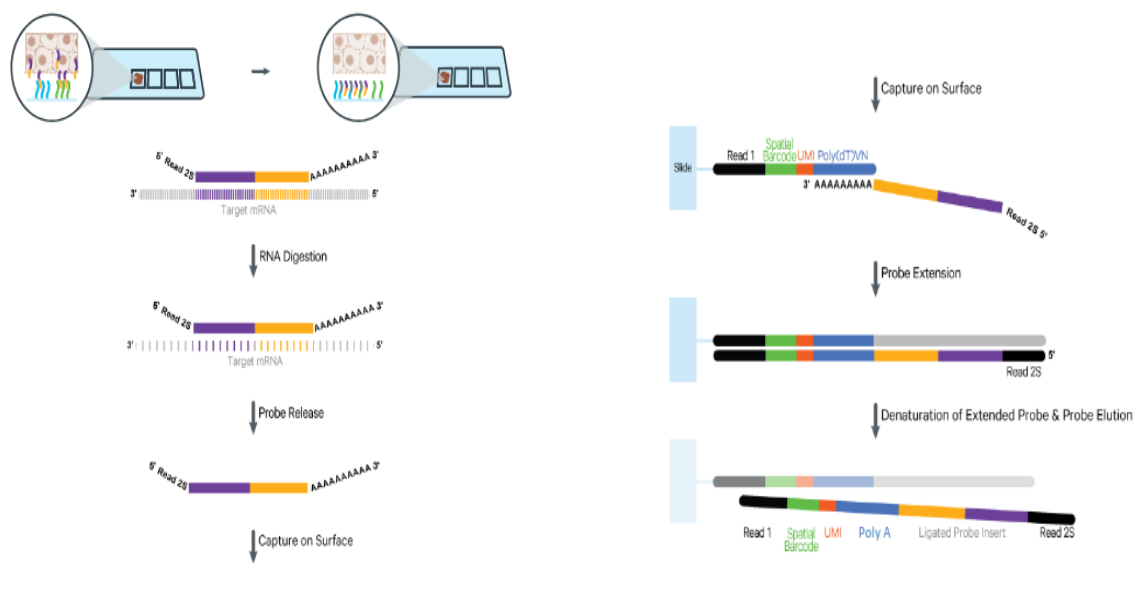
\includegraphics[width=\textwidth, height=6.2cm]{Images/ffpe_visium.png}
        \end{minipage}%
        \hfill
        \begin{minipage}{0.23\textwidth}
            \vspace{5.5cm}
            \raggedleft
            {\tiny \color{gray} Source: 10x Genomics}
        \end{minipage}
        \centering
        \textbf{Probe hybridization and ligation to capture RNA in each spots}
    \end{figure}
\end{frame}


\begin{frame}{RCTD deconvolution}
    \frametitle<presentation>{}
    
    \begin{figure}[h]
        \begin{minipage}{0.65\textwidth}
            \raggedleft
            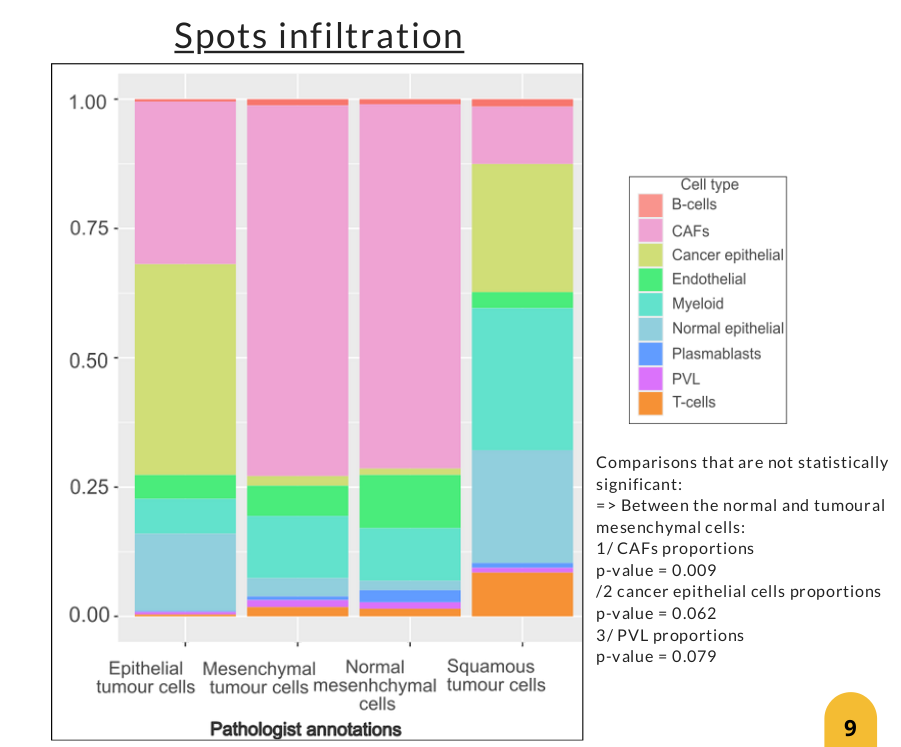
\includegraphics[width=\textwidth, height=6cm]{\figpath/Deconv_Ines.png}
        \end{minipage}

        \hfill

        \begin{minipage}{0.48\textwidth}
            \raggedleft
            \tiny \color{gray} Source: Ines Kardous M2 Internship 2024 
        \end{minipage}
    \end{figure}
\end{frame}

\begin{frame}{Xenium}
    \frametitle<presentation>{}
    
    \begin{figure}[h]
        \begin{minipage}{0.65\textwidth}
            \raggedleft
            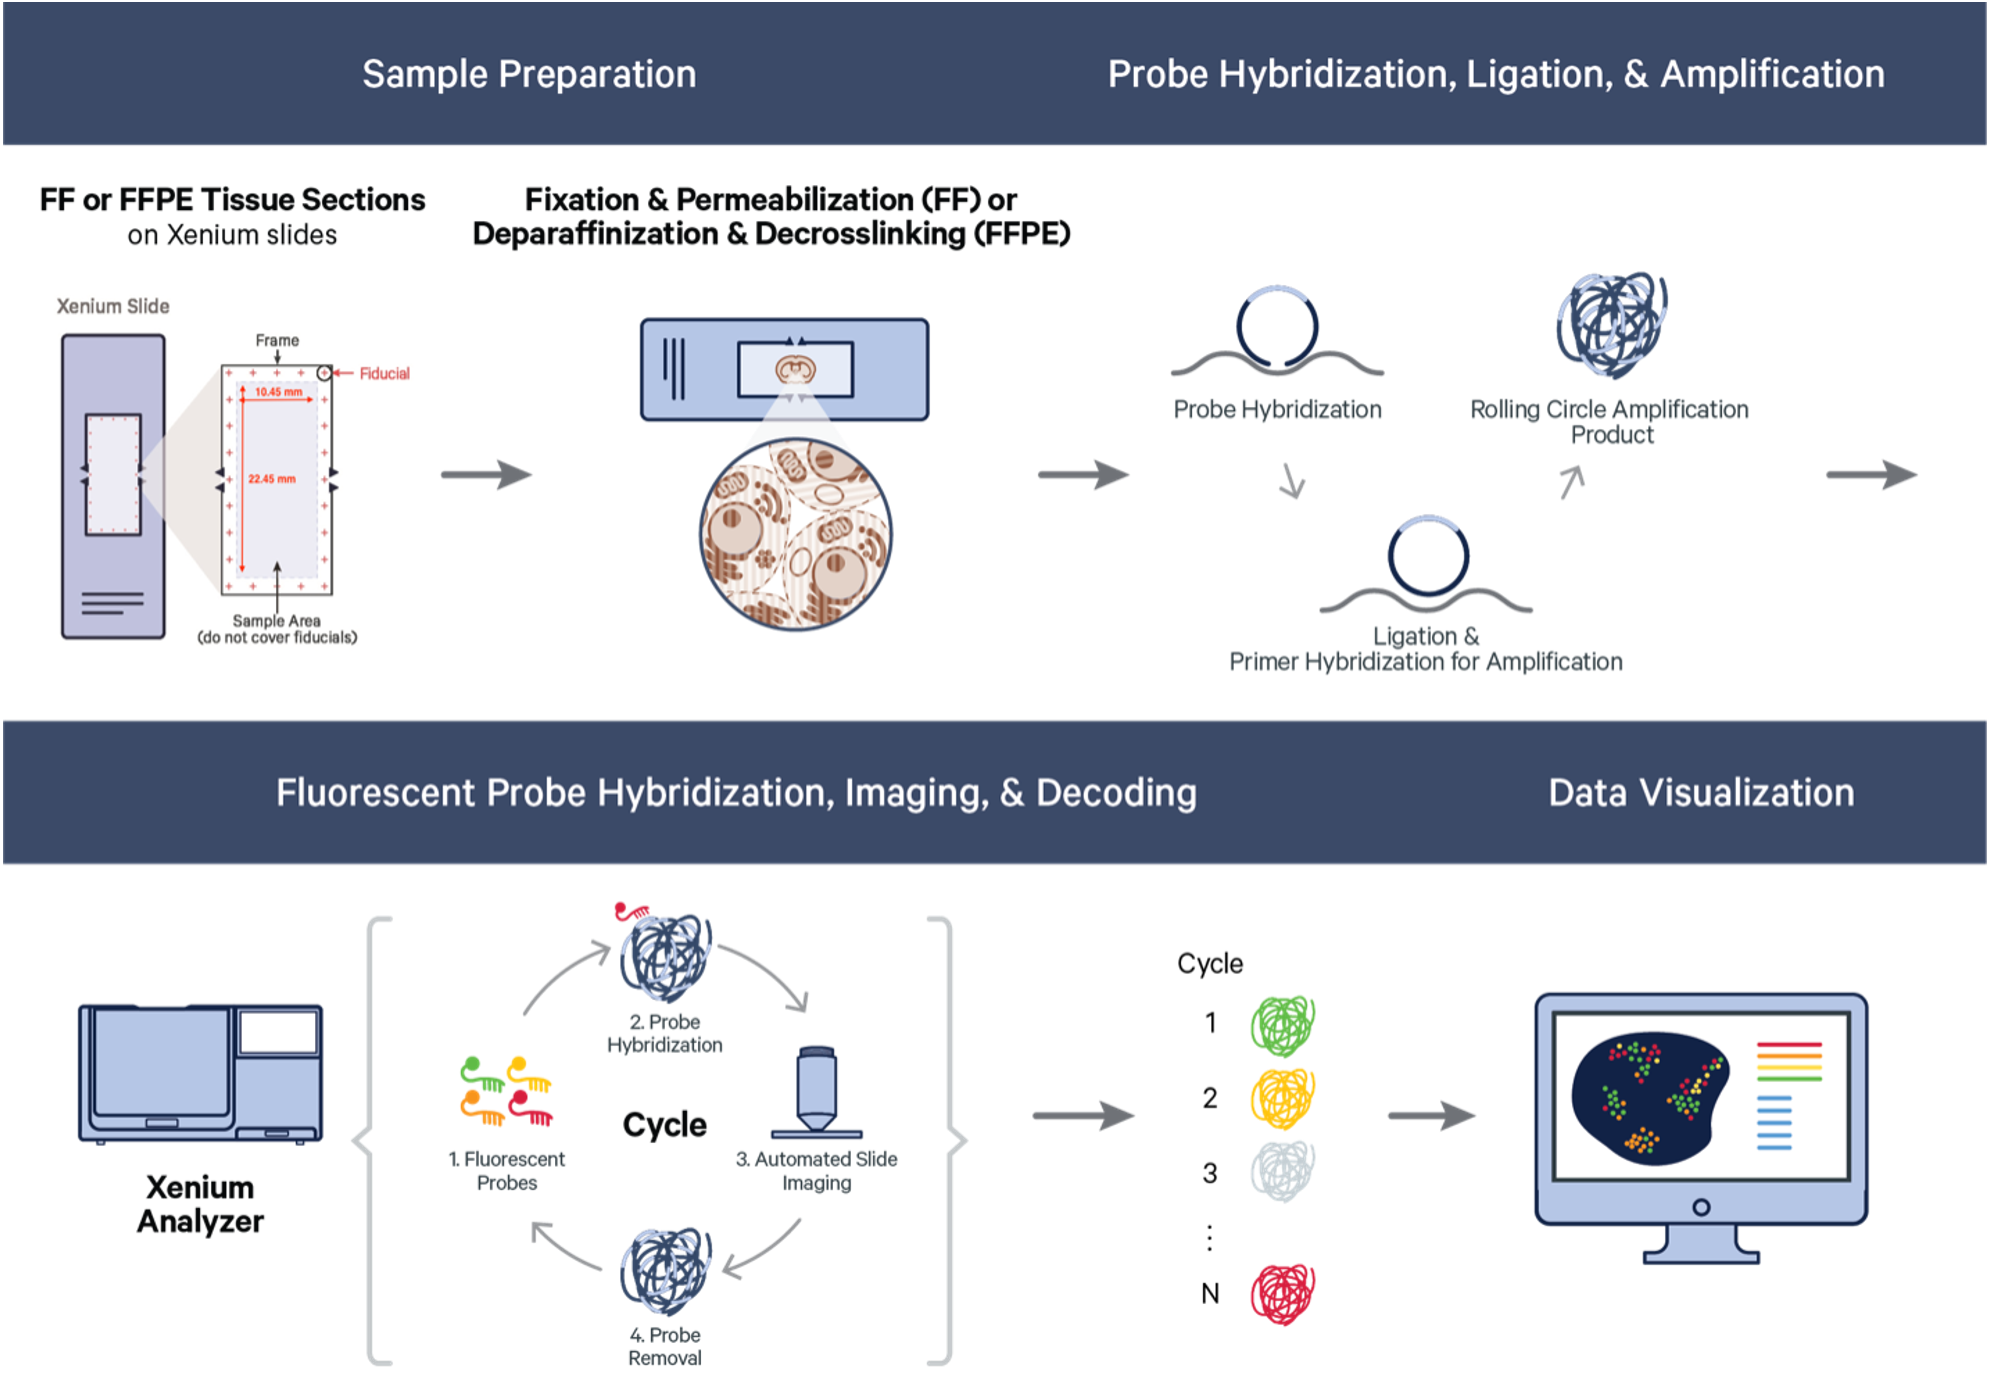
\includegraphics[width=\textwidth, height=6cm]{Images/xenium-workflow.png}
        \end{minipage}

        \hfill

        \begin{minipage}{0.48\textwidth}
            \raggedleft
            \tiny \color{gray} Source: 10x Genomics 
        \end{minipage}
    \end{figure}
\end{frame}

\end{document}